% !TEX root = ../00_tcc.tex

\begin{figure}[h]
	\centering
	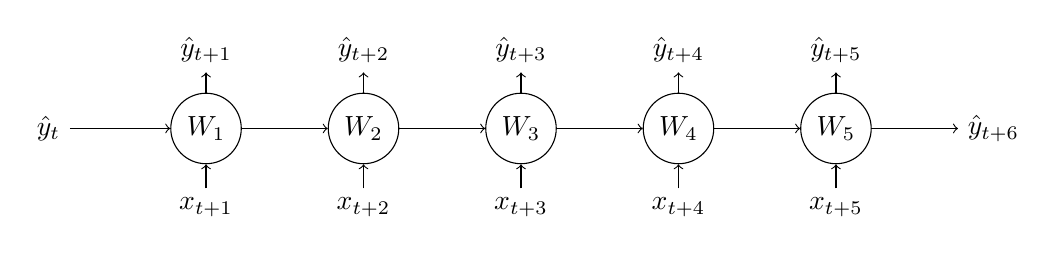
\begin{tikzpicture}
    \tikzstyle{neuron}=[circle, draw=black, minimum size = 8mm]

	\node[]       (n0)  at  (0,0)  {$\hat{y}_t$};
	\node[]       (y)   at  (12,0) {$\hat{y}_{t+6}$};

	\foreach \i in {1,...,5}{
		\node[]       (n\i1)  at  (\i*2,1)  {$\hat{y}_{t+\i}$};
		\node[neuron] (n\i2)  at  (\i*2,0)  {$W_\i$};
		\node[]       (n\i3)  at  (\i*2,-1) {$x_{t+\i}$};

		\draw[->]     (n\i2)  --  (n\i1)  ;
		\draw[->]     (n\i3)  --  (n\i2)  ;
		}

	\draw[->]     (n0)   --  (n12)  ;
	\draw[->]     (n12)  --  (n22)  ;
	\draw[->]     (n22)  --  (n32)  ;
	\draw[->]     (n32)  --  (n42)  ;
	\draw[->]     (n42)  --  (n52)  ;
	\draw[->]     (n52)  --  (y)    ;

	\end{tikzpicture}
	\caption{Representação de uma Rede Neural recorrente. Fonte: própria.}\label{tikz:rnn}
\end{figure}
